

\documentclass[crop,tikz]{standalone}% 'crop' is the default for v1.0, before it was 'preview'
\usepackage{tikz,calc,pgfplots}
\usetikzlibrary{calc}
\begin{document}
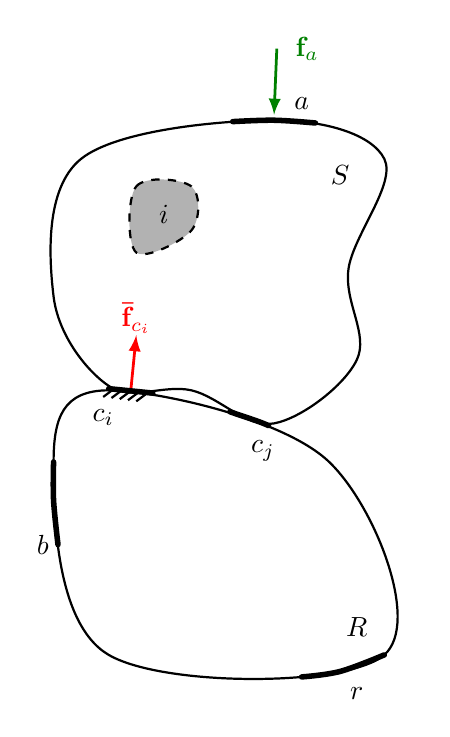
\begin{tikzpicture}[scale=0.7]


 \draw [thick]  plot[smooth cycle, tension=.6] coordinates {(0,2) (0.5,4.5) (4,5.2) (6,4.5)  (5.35,2.5) (5.5,0.85) (4,-0.3) (2.5,0.3) (1,0.38) };
 
\node[outer sep=0pt,thick] at (5.2,4.2) [] {${S}$};
 
\draw [thick,dashed, fill=white!70!black]  plot[smooth cycle,  tension=.6] coordinates {(1.5,2.8) (1.5,4) (2.5,4)  (2.5,3.2) };

\node[outer sep=0pt,thick] at (2,3.5) [] {$i$};
 
 
\draw [thick]  plot[smooth cycle, tension=.6] coordinates {(0,-1) (1,-4.5) (6,-4.5) (5,-1) (1,0.3) };
\node[outer sep=0pt,thick] at (5.5,-4) [] {${R}$};

\draw [line width=1pt,red,-latex]  plot[smooth, tension=.6] coordinates { (1.4,0.29)  (1.5,1.3) }; 
\node[outer sep=0pt,thick] at (1.5,1.6) [] {{\color{red}${\mathbf{\bar{f}}_{c_i}}$}};
 
\draw [line width=2pt,black,cap=round]  plot[smooth, tension=.6] coordinates { (3.2,-0.09) (3.7,-0.26) (3.9,-0.34) };  
\node[outer sep=0pt,thick] at (3.8,-0.8) [] {$c_j$};

\draw [line width=2pt,black,cap=round]  plot[smooth, tension=.6] coordinates { (1,0.33) (1.2,0.31) (1.8,0.25) };  
\node[outer sep=0pt,thick] at (0.9,-0.2) [] {$c_i$};



\draw [line width=1pt,green!50!black,-latex]  plot[smooth, tension=.6] coordinates { (4.05,6.5)  (4,5.3) }; 
\node[outer sep=0pt,thick] at (4.6,6.5) [] {{\color{green!50!black}$\mathbf{{f}}_{a}$}};

\draw [line width=0.8pt]  plot[smooth, tension=.6] coordinates { (1.1,0.33)  (0.9,0.18) }; 
\draw [line width=0.8pt]  plot[smooth, tension=.6] coordinates { (1.25,0.31)  (1.05,0.16) }; 
\draw [line width=0.8pt]  plot[smooth, tension=.6] coordinates { (1.4,0.29)  (1.2,0.14) }; 
\draw [line width=0.8pt]  plot[smooth, tension=.6] coordinates { (1.55,0.27)  (1.35,0.12) }; 
\draw [line width=0.8pt]  plot[smooth, tension=.6] coordinates { (1.7,0.25)  (1.5,0.10) }; 
%

%
%
\draw [line width=2pt,black,cap=round]  plot[smooth, tension=.6] coordinates { (3.25,5.175) (4,5.2) (4.75,5.15) };  
 \node[outer sep=0pt,thick] at (4.5,5.5) [] {$a$};
% 
% 
\draw [line width=2pt,black,cap=round]  plot[smooth, tension=.6] coordinates {  (6,-4.5) (5.2,-4.8) (4.5,-4.9) };  
\node[outer sep=0pt,thick] at (5.5,-5.2) [] {$r$};

%    \node at (-0.25,-4.3) {{(b)}}; 

    \draw [line width=2pt,black,cap=round]  plot[smooth, tension=.6] coordinates {  (0.08,-2.5) (0,-1.7) (0,-1) };  
\node[outer sep=0pt,thick] at (0.08,-2.5) [left] {$b$};
 \end{tikzpicture}
\end{document}